\chapter{INTRODUCTION}
We, as a society nowadays, are in constant demand for energy. Although,
even with the development of calculating, conducting and studying it, we
don't really know what the energy is, we are depending on that abstract
quantity. One might probably say that to study physics is to endure to
study energy in its every possible form. There's a brilliant quote from
Bill Bryson that: ``Energy is liberated matter, matter is energy waiting
to happen.'' What might be incredible is that from this strictly
mathematical quantity we can deduct anything. And what's also important
it is as arbitrary as it gets, depending only on one's reference. From
energy we can create few more important quantities such as \emph{power}
P, which is simply the energy provided per unit time, so:

$$E = \int P\left( t \right)dt$$

The energy will be represented in J (Joules) or eV (electron
volt), which directly describes energy of elementary charge
(\(e \approx 1.602*10^{- 19}C)\) in 1V (Volt) potential.

$$1eV = 1.602*10^{- 19}J$$

Power will be then represented in W (Watts) (\(W = \frac{J}{s}\ ).\)

The rise of energy consumption has proven that in the future we will
almost certainly require even more. From Global Energy Perspective paper 
\cite{Insights2019} we can learn that:

\begin{itemize}
\item Global energy demand will begin to reach a plateau at around 2035, despite a strong population expansion and economic growth, thanks to emphasis on renewable sources, more efficient service industries or more efficient industrial regions.
\item The energy demand and economic growth has became ``decoupled'' for the first time in history.
\item Renewable sources will provide more than half the electricity after 2035.
\end{itemize}

\noindent The reader is strongly recommended to take a look at the document.

\noindent With telling that we can produce energy there's a slick trick given with
the phrase. Energy cannot be simply created, it is just converted from
another source - so nothing is ever lost or miraculously made. The
problems we need to struggle with are then being able to obtain as much
energy from the energy source as it is possible. Of course, as
humankind society is governed by money, we need to keep the cost lowest simultaneously. There is plenty of different energy sources, that we have learned of, to receive energy
from. In Figure \ref{fig:ensour} we can see the most vivid ones nowadays. But with
the human demand fulfilment come great damages and soon depleting
resources of many energy sources such as fossil fuels.


\begin{figure}[H]
\centering
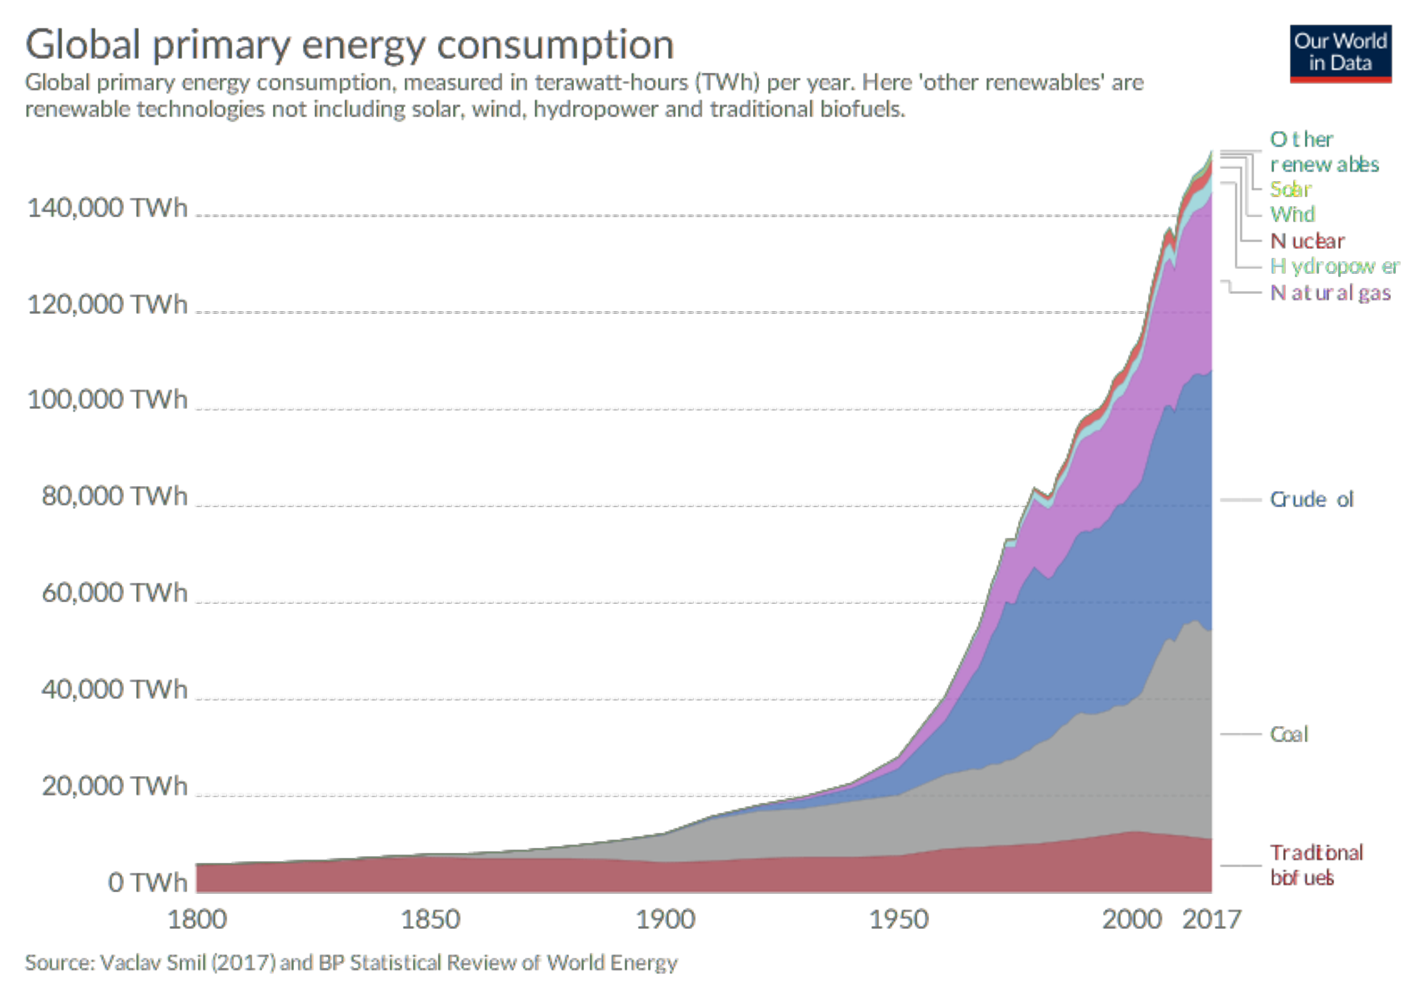
\includegraphics[width=0.6\textwidth]{global-primary-energy}
\caption{Energy sources contribution in world scale
\cite{2019}}
\label{fig:ensour}
\end{figure}

\noindent The necessity of searching new possible ways to harness it through renewable sources has become a global issue. Our concern of the environment had never been that serious before. Not only the change of methods for energy production must be enhanced because of this demand but we need to be strictly aware of the World's urging trepidation of Global Warming, of which evidence is provided for example here \cite{Nasa2019}.

\noindent Among all of the ideas created in a past few decades, solar energy is
believed by many to be one of the most reliable and promising. It can be
directly converted into electricity, heat or chemical energy and our
only Star seems to be an "infinite power" resource for us. In the last ten
years the world solar PV electricity production has grown impressively,
being almost three times bigger in 2016, than in 2010 \cite{2018}. In theory,
the Sun has the potential to fulfil earth's energy demand, if it is not
for the technology. Annually, nearly 10\textsuperscript{18} EJ of energy
reaches our planet and of that 10\textsuperscript{4} EJ is claimed to be
harvestable. The possibility of converting the solar energy into
electric energy has been studied since discovery of the basic
photovoltaic effect and the development of first semiconductor technologies.

Since the first crystalline silicon solar cell, the technology had undergone a vivid development. The number of different methods that the cell can be created with and the quantity of possible final outcomes isn't inconsiderable. Yet, solar cells can be classified into three generations in accordance to the development technology and materials used\cite{HuashangRao2018}. The first generation describes silicon based solar cells, which so far is the most researched type. It includes mono-crystalline and polycrystalline silicon cells.

The second generation contains thin film solar cells. It refers to amorphous silicon, copper indium gallium selenide (CIGS), GaAs and CdTe devices. With many advantages, such us direct band gaps resulting with harvesting light in very thin films, they still have a small share in the market of PV devices (<10\%) due to their instability and limitation in module technology\cite{HuashangRao2018}.

\begin{figure}[ht]
\label{fig:annual} 
\centering
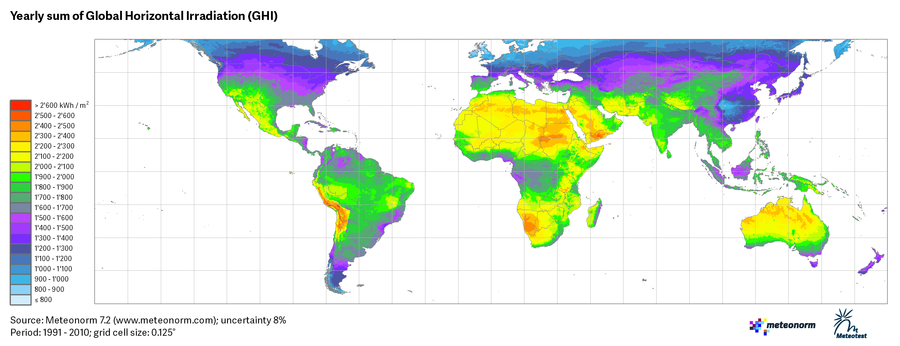
\includegraphics[width=\textwidth]{annual}
\caption{Annual yearly sum of Global Horizontal Irradiation
\cite{1991-2010}}
\end{figure}

The third generation cannot be simplified as much as it's formers. It is usually defined as solar cells that are still in scientific research phase\cite{HuashangRao2018} \cite{GavinCon}. It's main motivation is to achieve a higher efficiency using newly discovered physical phenomena, structures and materials. Their aim shall vary depending on the development technique and the physical principles. Today, the third generation mainly includes perovskite solar cells(PSCs) \cite{PerovRev} \cite{revPerold}, organic/polymer solar cells(OSCs) \cite{Polymer}, dye sensitized solar cells(DSCs)\cite{DyeSent} and quantum dot based solar cells(QDSC). \cite{Kamat2018} While still being considerably less common, the cons of investigating the nature and crucial properties of third generation PVs is overwhelming. Thanks to the ultimate specification of third generation approach, the devices can in perspective generate greater efficiency than other generations(for example by creating multiple electron-hole pairs and multi-band cells), yet while still being significantly cheaper than their formers.

\vline

Our main goal will be to study the QD sensitized solar cells and their characteristics. The base shall be put on PbS quantum dots as a light-harvesting material. We will proceed to consider their tunable band gap and other properties, such as control of composition, dipole moments, stability or collocation, and fit other materials to study the effects and their attributes. In principle, the QD solar cells can be distributed into four different classes: Schottky junction solar cells, p-n junction solar cells, hybrid QD-polymer solar cells and \textbf{quantum dot-sensitized solar cells (QDSCs)} and this is yet to be found later on...